\documentclass{scrartcl}

\usepackage[utf8]{inputenc}
\usepackage[T1]{fontenc}
\usepackage{lmodern}
\usepackage[ngerman]{babel}
\usepackage{amsmath}

\usepackage{hyperref}

\usepackage[justification=RaggedRight, singlelinecheck=false]{caption}
\usepackage{subcaption} 

\usepackage{listings}
\usepackage[usenames,dvipsnames]{xcolor}

% This is the color used for MATLAB comments below
\definecolor{MyDarkGreen}{rgb}{0.0,0.4,0.0}

% For faster processing, load Matlab syntax for listings

\lstloadlanguages{Matlab}%

\lstset{language=Matlab,                        % Use MATLAB
        frame=single,                           % Single frame around code
        basicstyle=\small\ttfamily,             % Use small true type font
        keywordstyle=[1]\color{Blue}\bfseries,        % MATLAB functions bold and blue
        keywordstyle=[2]\color{Purple},         % MATLAB function arguments purple
        keywordstyle=[3]\color{Blue}\underbar,  % User functions underlined and blue
        identifierstyle=,                       % Nothing special about identifiers
                                                % Comments small dark green courier
        commentstyle=\usefont{T1}{pcr}{m}{sl}\color{MyDarkGreen}\small,
        stringstyle=\color{Purple},             % Strings are purple
        showstringspaces=false,                 % Don't put marks in string spaces
        tabsize=5,                              % 5 spaces per tab
        %
        %%% Put standard MATLAB functions not included in the default
        %%% language here
        morekeywords={xlim,ylim,var,alpha,factorial,poissrnd,normpdf,normcdf},
        %
        %%% Put MATLAB function parameters here
        morekeywords=[2]{on, off, interp},
        %
        %%% Put user defined functions here
        morekeywords=[3]{FindESS, homework_example},
        %
        morecomment=[l][\color{Blue}]{...}    % Line continuation (...) like blue comment
}

% Includes a MATLAB script.
% The first parameter is the label, which also is the name of the script
%   without the .m.
% The second parameter is the optional caption.
\newcommand{\matlabscript}[2]
  {\begin{itemize}\item[]\lstinputlisting[caption=#2,label=#1]{#1.m}\end{itemize}}

\usepackage[edges]{forest}
\usetikzlibrary{shadows}
\definecolor{folderbg}{RGB}{124,166,198}
\definecolor{folderborder}{RGB}{110,144,169}

\newlength\Size
\setlength\Size{4pt}
\tikzset{%
  folder/.pic={%
    \filldraw [draw=folderborder, top color=folderbg!50, bottom color=folderbg] (-1.05*\Size,0.2\Size+5pt) rectangle ++(.75*\Size,-0.2\Size-5pt);
    \filldraw [draw=folderborder, top color=folderbg!50, bottom color=folderbg] (-1.15*\Size,-\Size) rectangle (1.15*\Size,\Size);
  },
  file/.pic={%
    \filldraw [draw=folderborder, top color=folderbg!5, bottom color=folderbg!10] (-\Size,.4*\Size+5pt) coordinate (a) |- (\Size,-1.2*\Size) coordinate (b) -- ++(0,1.6*\Size) coordinate (c) -- ++(-5pt,5pt) coordinate (d) -- cycle (d) |- (c) ;
  },
}

\forestset{%
  declare autowrapped toks={pic me}{},
  declare boolean register={pic root},
  pic root=0,
  pic dir tree/.style={%
    for tree={%
      folder,
      font=\ttfamily,
      grow'=0,
    },
    before typesetting nodes={%
      for tree={%
        edge label+/.option={pic me},
      },
      if pic root={
        tikz+={
          \pic at ([xshift=\Size].west) {folder};
        },
        align={l}
      }{},
    },
  },
  pic me set/.code n args=2{%
    \forestset{%
      #1/.style={%
        inner xsep=2\Size,
        pic me={pic {#2}},
      }
    }
  },
  pic me set={directory}{folder},
  pic me set={file}{file},
}

\usepackage{graphicx,import}
\usepackage{transparent}
\usepackage{float}

\title{Handbuch}
\author{Benjamin Schnabel}
\date{\today}

\begin{document}

\maketitle
\tableofcontents

\section{Verzeichnisstruktur}

In Abbildung \ref{fig:verzeichnisstruktur} ist eine Übersicht über die Verzeichnisstruktur des Modells zur Simulation der thermischen Eigenschaften beim Selektiven Lasersintern dargestellt. Im Folgenden werden nur die für die Durchführung der Simulation wichtigsten Funktionen erklärt.

\begin{figure}[H]
\begin{forest}
pic dir tree,
pic root,
for tree={
	directory,
},
[\textbackslash
[{\hyperref[sec:laserModel]{Laser model}}
[{\hyperref[subsec:getLaserParameter]{getLaserParameter.m}}, file]
]
[{\hyperref[sec:latex]{Latex}}]
[{\hyperref[sec:materialModel]{Material model}}]
[{\hyperref[sec:plots]{Plots}}]
[{\hyperref[sec:reports]{Reports}}]
[{\hyperref[sec:stlFile]{STL file}}]
[{\hyperref[sec:thermalModel]{Thermal model}}
[{\hyperref[subsec:getThermalParameter]{getThermalParameter.m}}, file]
]
[{\hyperref[sec:usefulFunctions]{Useful functions}}
[{\hyperref[subsec:plotSimulation]{plotSimulation.m}}, file]
]
[{\hyperref[sec:main]{main.m}}, file]
]
\end{forest}
\caption{Verzeichnisstruktur}
\label{fig:verzeichnisstruktur}
\end{figure}

\section{Schnellstart}\label{sec:schnellstart}

Für den Schnellstart der Simulation wird die STL-Datei im Ordner \textit{STL file} abgelegt. Im Anschluss wird die Matlab-Datei \textit{main.m} geöffnet und über den Befehl \textit{Run main} bzw. über die Taste \textit{F5} gestartet. In Abbildung \ref{fig:1} ist der Auswahldialog der STL-Datei dargestellt. In diesem wird einfach die zuvor abgelegte Datei ausgewählt. Im nächsten Schritt werden noch die wichtigsten Simulationsparameter abgefragt. Dies ist in Abbildung \ref{fig:2} dargestellt. 

\begin{figure}[H]
\centering
\begin{subfigure}[t]{0.4\textwidth}
\centering
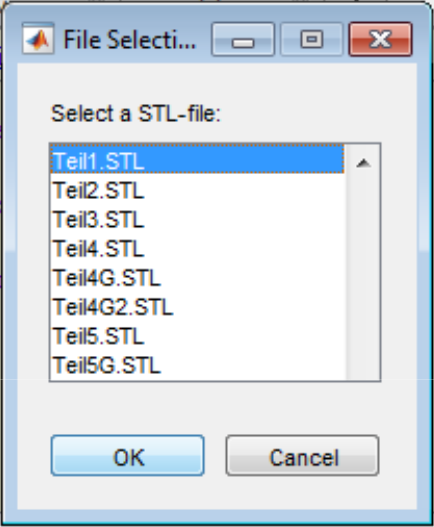
\includegraphics[width=\textwidth]{bild2.png}
\caption{STL-Datei Auswahldialog}
\label{fig:1}
\end{subfigure}
\begin{subfigure}[t]{0.55\textwidth}
\centering
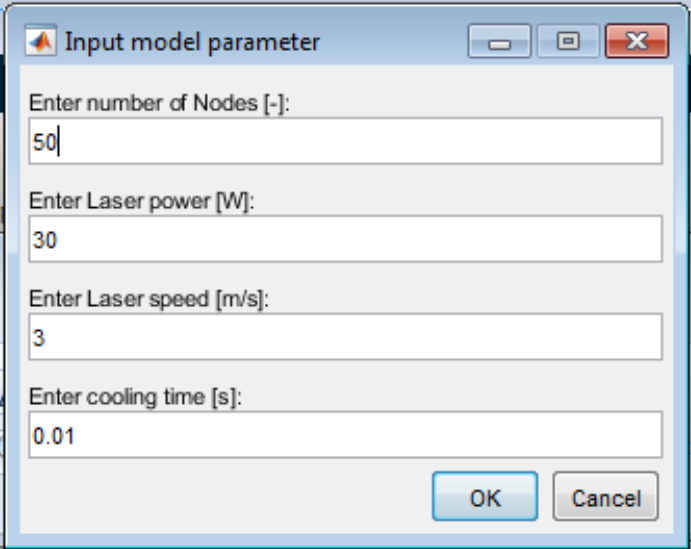
\includegraphics[width=\textwidth]{bild1.png}
\caption{Parametereingabe}
\label{fig:2}
\end{subfigure}
\caption{Eingabefenster}
\end{figure}

\section{main.m}\label{sec:main}

Main-Funktion zur Ausführung der Simulation. Im Folgenden werden nur die Module (Funktionen) beschrieben, die eine Auswahlmöglichkeit bieten.

\subsection{Wärmestromdichte grafisch darstellen}

Erstellte Datei wird im Ordner {\hyperref[sec:plots]{Plots}} abgelegt.

\begin{lstlisting}
% Display the heat flux intensity in a figure (true or false)
displayHeatFluxIntensityFigure = 'false';
switch displayHeatFluxIntensityFigure
    case 'true'
        % exportAsPDF (true or false)
        plotHeatFluxIntensity(0.02, 'false', P, r_0, r_w);
    case 'false'
    otherwise
        disp('Error: displayHeatFluxIntensityFigure')
end
\end{lstlisting}

\subsection{Drehung des Voxel-Modells}

\begin{lstlisting}
% Rotate Voxel- Matrix along z axis
rotateZAxis = '0';

switch rotateZAxis
    case '0'
        voxelModel = rot90(voxelModel,0);
    case '90'
        voxelModel = rot90(voxelModel,1);
    case '180'
        voxelModel = rot90(voxelModel,3);
    case '270'
        voxelModel = rot90(voxelModel,2);
    otherwise 
        disp('Error: rotateZAxis')
end
\end{lstlisting}

\subsection{Voxel-Modell grafisch darstellen}

Erstellte Datei wird im Ordner {\hyperref[sec:plots]{Plots}} abgelegt.

\begin{lstlisting}
% Display the voxel model in a figure (true or false)
displayVoxelModelFigure = 'false';
switch displayVoxelModelFigure
    case 'true'
        % exportAsPDF (true or false)
        plotVoxelModel(voxelModel, n, 'false');
    case 'false'
    otherwise
        disp('Error: displayVoxelModelFigure')
end
\end{lstlisting}

\subsection{Video der Simulation erstellen}

\begin{lstlisting}
% Create a movie plot (true or false)
createVideoPlot = 'false';
switch createVideoPlot
    case 'true'
        plotSimulationForVideoExport(TemperatureArray, ...
            n, n_new, x, y, z, xSliced, ySliced, region, ...
            stlFileNameShortened, fileDate);
    case 'false'
    otherwise
        disp('Error: createVideoPlot')
end
\end{lstlisting}

\subsection{Eigenwerte der Temperaturmatrix bestimmen}

\begin{lstlisting}
% Create a plot of the eigenvalues (true or false)
createEigenvaluesPlot = 'true';
switch createEigenvaluesPlot
    case 'true'
        % exportAsPDF (true or false)
        fig = plotEigenvalues(TemperatureArray, 'true', ...
            stlFileNameShortened, fileDate);
    case 'false'
    otherwise
        disp('Error: createEigenvaluesPlot')
end
\end{lstlisting}

\subsection{Excel-Datei als Latex Tabelle exportieren}

\begin{lstlisting}
% Export excel-file as Latex table
createLatexTable = 'false';
switch createLatexTable
    case 'true'
        exportAsLatexTable(fileName)
    case 'false'
    otherwise
        disp('Error: createLatexTable')
end
\end{lstlisting}

\section{Laser model}\label{sec:laserModel}

In diesem Ordner sind alle Funktionen zur Beschreibung der Wärmestromdichte eines Gauß-Laserstrahls für eine TEM$_{00}$-Mode abgelegt.

\subsection{getLaserParameter}\label{subsec:getLaserParameter}

In dieser Funktionen können die Parameter zur Beschreibung des Lasers vordefiniert werden. Alle in Abbildung \ref{fig:2} definierten Parameter werden aus dieser Funktion ausgelesen. 

\begin{lstlisting}
function parameter = getLaserParameter()
    % Stefan-Boltzmann constant [W/(m^2 K^4)]
    parameter.stefanBoltzmanConstant = 5.670367 * 10^-8;
    % Focal length [mm]
    parameter.focalLength = 120.0;
    % Wave length [ym]
    parameter.waveLength = 10.63;
    % Laser power [W]
    parameter.laserPower = 30.0;
    % Raw beam radius at focusing lens [mm]
    parameter.rawBeamRadius = 16.0;
    % Distance to focal point [mm]
    parameter.distanceFocalPoint  = 10.0;
    % Laser Speed [m/s]
    parameter.laserSpeed = 3.0;
end
\end{lstlisting}

\section{Latex}\label{sec:latex}

\section{Material model}\label{sec:materialModel}

In diesem Ordner sind alle Funktionen zur Beschreibung der Eigenschaften des Werkstoffes abgelegt. Dies beinhaltet die spezifische Wärmekapazität $ c_{p} $, Wärmeleitfähigkeit $ \kappa $, Dichte $ \rho $ und Temperaturleitfähigkeit $ a $.

\section{Plots}\label{sec:plots}

\section{Reports}\label{sec:reports}

Nach jeder Simulation werden die erstellten Berichte in diesem Ordner automatisch abgelegt.

\section{STL file}\label{sec:stlFile}

Die erstellen STL-Dateien werden in diesem Ordner abgelegt.

\section{Thermal model}\label{sec:thermalModel}

In diesem Ordner ist die Funktion zur Berechung der Wärmeübertragung, die Implementierung des Explizites Euler-Verfahrens und die Funktion zum Vordefinieren der thermischen Parameter abgelegt.

\subsection{getThermalParameter}\label{subsec:getThermalParameter}

In dieser Funktionen können die Parameter zur Beschreibung des thermischen Eingenschaften vordefiniert werden. Die Anzahl der Gitterpunkte und die Abkühlungszeit pro Schicht (siehe Abbildung \ref{fig:2}) werden aus dieser Funktion ausgelesen. 

\begin{lstlisting}
function parameter = getThermalParameter()
    % Number of nodes
    parameter.numberOfNodes = 25;
    % Chamber temperature [K]
    parameter.chamberTemperature = 273.15 + 175.0;
    % Powderbed temperature [K]
    parameter.powderbedTemperature = 273.15 + 163.0;
    
    % Boltzmann constant [J/K]
    parameter.boltzmannConstant = 1.3806504 * 10^-23;
    % Speed of light [m/s]
    parameter.speedOfLight = 299792458;
    % Planck constant [Js]
    parameter.planckConstant = 6.62606896 * 10^-34;
    
    % Cooling time [s]
    parameter.coolingtime = 0.01;
end
\end{lstlisting}

\section{Useful functions}\label{sec:usefulFunctions}

\subsection{plotSimulation}\label{subsec:plotSimulation}

Die Transparenz kann über den Befehl \textit{alpha(h,0.2)} angepasst werden, wobei der Wert nach dem \textit{h} die Transparenz bestimmt.

\begin{lstlisting}
function [fig] = plotSimulation(fin, x, y, z, xSliced,  ...)
    
    fig = figure(1);
    fin(fin == 0) = NaN;
    h = slice(x,y,z,fin-273.15,xSliced,ySliced,Inf);
    axis(region);
    set(h,'EdgeColor','none')
    set(gca,'xtick',[])
    set(gca,'ytick',[])
    set(gca,'ztick',[])
    xlabel('x')
    ylabel('y')
    zlabel('z')
    cb = colorbar;
    ylabel(cb, '{}^{\circ}C', 'Interpreter','tex')
    alpha(h,0.2);
    set(gca,'fontsize',12)
    
    stlName = stlName(1:end-4);
    fileName = [stlName, '-Layer', num2str(i)];
    orient(fig,'landscape')
    print(fig,'-bestfit',fileName,'-dpdf','-r0')
end
\end{lstlisting}

\section{Ablauf Simulation}

\begin{figure}[H]
\centering
\def\svgwidth{350pt}
\input{Programmablaufplan.pdf_tex}
\caption{Programmablaufplan zur Durchführung der Simulation}
\label{fig:softwareablauf}
\end{figure}

\end{document}